% Chapter 1

\chapter{Introducción general} % Main chapter title

\label{Chapter1} % For referencing the chapter elsewhere, use \ref{Chapter1} 
\label{IntroGeneral}

%----------------------------------------------------------------------------------------

% Define some commands to keep the formatting separated from the content 
\newcommand{\keyword}[1]{\textbf{#1}}
\newcommand{\tabhead}[1]{\textbf{#1}}
\newcommand{\code}[1]{\texttt{#1}}
\newcommand{\file}[1]{\texttt{\bfseries#1}}
\newcommand{\option}[1]{\texttt{\itshape#1}}
\newcommand{\grados}{$^{\circ}$}

%----------------------------------------------------------------------------------------

%\section{Introducción}

En este capítulo se presenta una introducción al concepto de aeroponía y sus principales ventajas. Además, se describe el estado del arte y se exponen los objetivos, alcance y requerimientos del trabajo.


%----------------------------------------------------------------------------------------
\section{Aeroponía}

La aeroponía es una técnica de cultivo de plantas en la que las raíces cuelgan suspendidas en el aire mientras se les entrega una solución nutritiva en forma de una fina niebla \citep{WEBSITE:AEROPONIA1}. Como se usa agua para transmitir nutrientes, a veces se habla de los cultivos aeropónicos como de tipo hidropónico \citep{WEBSITE:HIDROPONIA}.

En la figura \ref{fig:zonaDeCultivoAeroponica} se presenta un típico ejemplo de una zona de cultivo aeropónica, en la que se puede observar el posicionamiento de las plantas y su sistema de nebulización.

\begin{figure}[htbp]
	\centering
	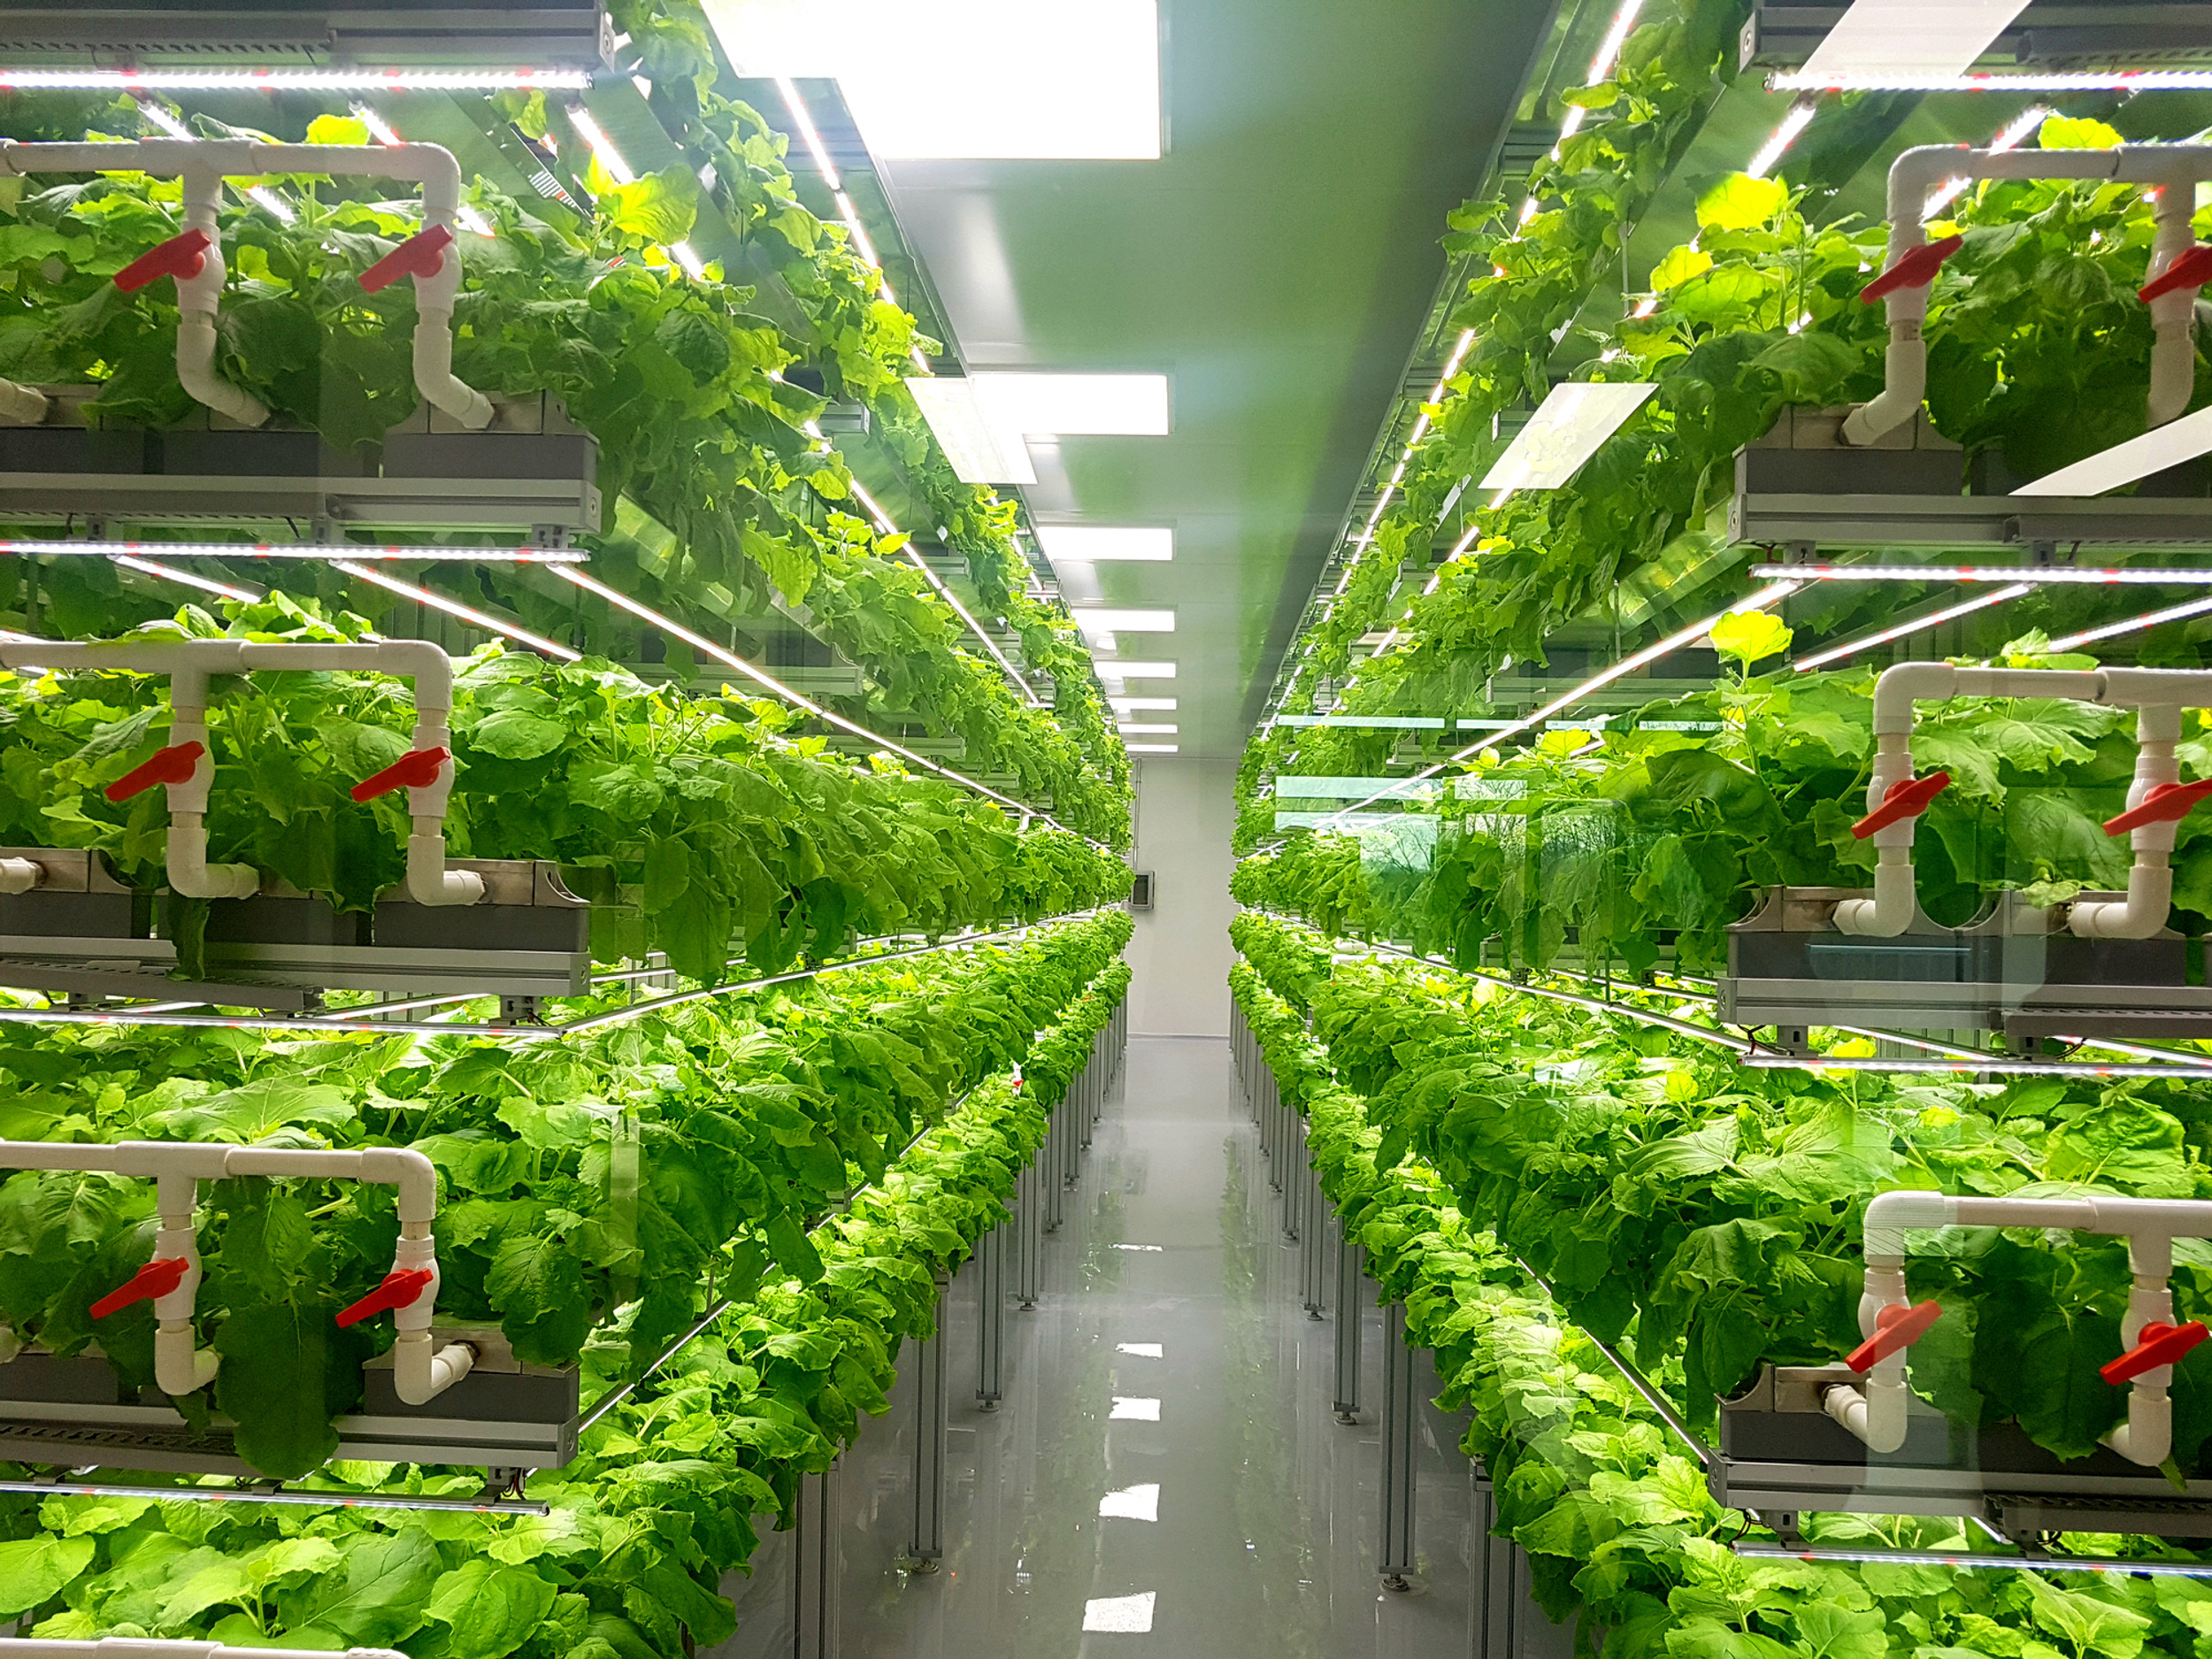
\includegraphics[width=.9\textwidth]{./Figures/Zona de cultivo aeroponica.jpg}
	\caption{Zona de cultivo aeropónica\protect\footnotemark.}
	\label{fig:zonaDeCultivoAeroponica}
\end{figure}


\footnotetext{Imagen tomada de \url{https://www.acquagarden.com.ar/aeroponia}}

El crecimiento aeropónico es considerado seguro y ecológico por producir cosechas de forma natural manteniendo las plantas saludables. Su principal ventaja ecológica frente a otros sistemas es la conservación de agua, energía y nutrientes  \citep{WEBSITE:AEROPONIA2}. 

Una de sus características más importante es que requieren poco contacto físico con el sistema radicular del cultivo, para no interferir con el crecimiento y expansión natural de las raíces y lograr un intercambio limpio de agua y aire. Por esta razón, en comparación con las plantas hidropónicas, los cultivos tienden a crecer más rápido y a absorber más nutrientes, ya que están expuestas a más oxígeno. A su vez, hay menos amenazas de enfermedades alrededor de la zona de la raíz ya que no hay lugar para que residan los desechos \citep{WEBSITE:AEROPONIA3}.

En la figura \ref{fig:diagramaAeroponia} puede observarse el diagrama de un cultivo aeropónico junto con su proceso de nebulización. 

\begin{figure}[htbp]
	\centering
	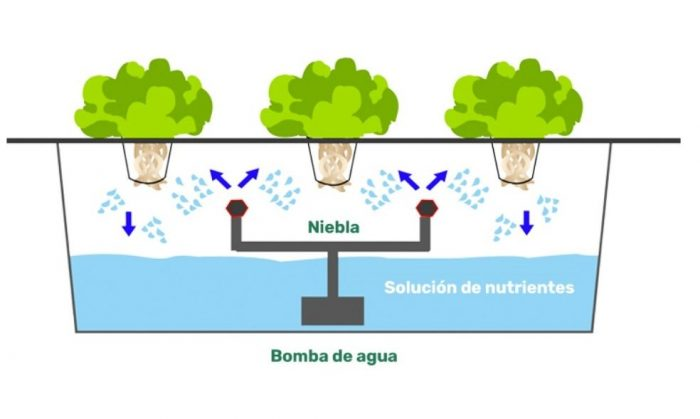
\includegraphics[width=.9\textwidth]{./Figures/Diagrama Aeroponia.jpg}
	\caption{Diagrama aeroponía\protect\footnotemark.}
	\label{fig:diagramaAeroponia}
\end{figure}

\footnotetext{Imagen tomada de \url{https://hidroponia24.com/sistemas-hidroponicos/aeroponia/}}

Sin embargo, para lograr que un sistema aeropónico tenga éxito es necesario que se controlen múltiples parámetros que son vitales para el correcto desarrollo de los cultivos, como por ejemplo la temperatura y caudal de la solución nutritiva a utilizar en el proceso de nebulización, la temperatura y humedad del ambiente, el nivel de dióxido de carbono y el nivel de iluminación entre otros \citep{WEBSITE:AEROPONIA4}.

%----------------------------------------------------------------------------------------

\section{Objetivos y alcance}

El propósito de este trabajo es el diseño, desarrollo e implementación de un sistema que permita la gestión de cultivos aeropónicos, con el objetivo de incrementar su productividad y reducir la dificultad de mantenimiento.

El trabajo incluye:
\begin{itemize}
	\item Diseño y desarrollo de una aplicación SSR (del inglés \textit{server-side rendering}) \citep{WEBSITE:SSR} que permita la interacción del usuario con el sistema.
	\item Diseño y desarrollo de una API (del inglés \textit{application programming interface}) \citep{WEBSITE:API} REST (del inglés \textit{representational state transfer}) \citep{WEBSITE:REST} que permita la comunicación por medio de los protocolos HTTP (del inglés \textit{Hypertext Transfer Protocol}) \citep{WEBSITE:HTTP}, MQTT (del inglés \textit{Message Queue Telemetry Transport}) \citep{WEBSITE:MQTT} y WebSocket \citep{WEBSITE:WEBSOCKET}.
	\item Diseño de un modelo de datos a utilizar por el DaaS (del inglés \textit{data as a service}) \citep{WEBSITE:DAAS} que permita almacenar los datos.
	\item Configuración y despliegue del DaaS.
	\item Diseño y desarrollo de un \textit{broker} que permita la comunicación por medio de los protocolos MQTT y WebSockets.
	\item Desarrollo del \emph{software} del microcontrolador para realizar una prueba de concepto.
\end{itemize}

El trabajo no incluye:
\begin{itemize}
	\item Diseño de un gabinete para el microcontrolador y los sensores a utilizar.
	\item Desarrollo del \emph{software} final del microcontrolador.
	\item Uso de certificados TLS (del inglés \textit{Transport Layer Security}) \citep{WEBSITE:TLS} emitidos por autoridades de confianza.
	\item Despliegue del servidor en un entorno \textit{cloud}.
	\item Accionar la bomba y el nebulizador del cultivo aeropónico por medio del sistema.
\end{itemize}

%----------------------------------------------------------------------------------------

\section{Estado del arte}

Se llevó a cabo una búsqueda de sistemas similares en el mercado nacional, pero solo se encontró un producto que ofrece características comparables o que cuente con documentación suficiente para una comparación adecuada. Por este motivo, se decidió incluir en la búsqueda sistemas del mercado internacional y publicaciones científicas. 

En la tabla \ref{tab:comparativaSolucionesNacionalesInternacionales} se presenta la comparación de las características y funcionalidades de los sistemas comerciales encontrados en el mercado nacional e internacional.

My Autogrow \citep{WEBSITE:MYAUTOGROW} permite la automatización y control de todo tipo de sistemas agrícolas. Los datos del sistema son obtenidos por medio de sensores y se almacenan en una plataforma \emph{cloud}. El sistema utiliza MQTT y HTTP como protocolos de comunicación. Los usuarios acceden al sistema mediante una aplicación web, cuyas principales características se detallan a continuación: 

\begin{itemize}
	\item Histórico de mediciones con filtros.
	\item Administración de alertas.
	\item Administración de áreas de cultivo.
	\item Administración de sistema de fertirrigación \citep{WEBSITE:FERTIRRIGACION}.
	\item Administración de sistema de riego.
	\item Visualización de gráficos.
\end{itemize}

Smartcultiva \citep{WEBSITE:PLIOT} permite la obtención de datos y métricas mediante una red de sensores instalados en la zona de cultivo. Los datos son enviados mediante MQTT y se almacenan en una plataforma \emph{cloud}. Los usuarios acceden al sistema mediante una aplicación web o móvil, cuyas principales características se detallan a continuación: 

\begin{itemize}
	\item Histórico de mediciones con filtros.
	\item Administración de dispositivos externos.
	\item Exportación de datos a diferentes formatos.
	\item Administración de alertas.
	\item Automatización de acciones frente al disparo de alertas.
	\item Visualización de gráficos.
\end{itemize}

Es importante notar que My Autogrow y Smartcultiva trabajan con sensores propietarios solamente.

\begin{table}[H]
	\centering
	\caption[Comparativa entre soluciones comerciales similares]{Comparativa entre soluciones comerciales similares.}
	\begin{tabular}{l c c c}    
		\toprule
		\textbf{Funcionalidad} & \textbf{Smartcultiva} & \textbf{My Autogrow} \\
		\midrule
		MQTT & Sí & Sí \\
		Sistema de alertas & Sí & Sí \\
		Acciones automatizadas & Sí & No \\
		Notificaciones \emph{push} \citep{WEBSITE:NOTIFICACIONESPUSH} & No & No \\
		Notificaciones \textit{email} & Sí & Sí \\
		Accionamiento de dispositivos externos & Sí & No \\
		Escalabilidad en sensores & Limitado & Limitado \\
		Tipo de aplicación & Móvil y web & Web \\
		\bottomrule
		\hline
	\end{tabular}
	\label{tab:comparativaSolucionesNacionalesInternacionales}
\end{table}

En la tabla \ref{tab:comparativaSolucionesPublicacionesCientificas} se presenta la comparación de las características y funcionalidades de los sistemas encontrados en publicaciones científicas.

\emph{Monitoring Soil and Ambient Parameters in the IoT Precision Agriculture Scenario: An Original Modeling Approach Dedicated to Low-Cost Soil Water Content Sensors} \citep{WEBSITE:SOLUCIONSIMILARCIENTIFICA2} presenta el desarrollo de un sistema de monitoreo de parámetros ambientales y del suelo enfocado en la agricultura. Los datos del sistema son obtenidos por nodos a nivel planta y a nivel de invernadero y enviados a un \emph{gateway} mediante el protocolo LoRa (del inglés \textit{long range}) \citep{WEBSITE:LORA}. El \emph{gateway} es el encargado de utilizar MQTT para enviar los datos a una plataforma \emph{cloud}. Los usuarios acceden al sistema mediante una plataforma web que permite monitorear los datos obtenidos y visualizar gráficos.

\emph{A Smart Agricultural System Based on PLC and a CloudComputing Web Application Using LoRa and LoRaWan} \citep{WEBSITE:SOLUCIONSIMILARCIENTIFICA3} presenta el desarrollo de un sistema compuesto por dos tipos de nodos: a nivel granja y a nivel depósito. Los nodos envían los datos obtenidos a un \emph{gateway} mediante el protocolo LoRa. El \emph{gateway} es el encargado de enviar los datos a una plataforma \emph{cloud}. Los usuarios acceden al sistema mediante una plataforma web que permite monitorear y exportar los datos obtenidos, administrar el sistema de alertas y visualizar gráficos. El sistema envía las notificaciones de las alertas mediante \textit{email} y un \textit{bot} \citep{WEBSITE:BOT} de Telegram \citep{WEBSITE:TELEGRAM}.

Se considera que la escalabilidad para incorporar nuevos sensores en las dos soluciones anteriores es media, debido a las estructuras planteadas a nivel aplicación. 

Es importante destacar que ambas soluciones fueron ejecutadas y probadas, es decir no son publicaciones teóricas. 

\begin{table}[H]
	\centering
	\caption[Comparativa entre soluciones similares encontradas en publicaciones científicas]{Comparativa entre soluciones similares encontradas en publicaciones científicas.}
	\begin{tabular}{l c c}    
		\toprule
		\textbf{Funcionalidad} & \textbf{\textit{Monitoring Soil (...)}} & \textbf{\textit{A Smart (...)}}  \\
		\midrule
		MQTT & Sí & No  \\
		LoRa & Sí & Sí  \\
		Sistema de alertas & No & Sí \\
		Acciones automatizadas & No & No \\
		Notificaciones \emph{push} & No & No \\
		Notificaciones \textit{email} & No & Sí \\
		Accionamiento de dispositivos externos & No & No \\
		Escalabilidad en sensores & Media & Media \\
		Tipo de aplicación & Web & Web \\
		\bottomrule
		\hline
	\end{tabular}
	\label{tab:comparativaSolucionesPublicacionesCientificas}
\end{table}

%----------------------------------------------------------------------------------------

\section{Requerimientos}

Se organizaron los requerimientos en secciones de acuerdo con su relación a las distintas áreas del trabajo.

\begin{enumerate}

	\item Requerimientos asociados a la aplicación SSR:
		\begin{enumerate}
			\item Deberá estar configurada para utilizar certificados TLS.
			\item Deberá estar configurada para poder enviar y recibir información mediante los protocolos HTTP y WebSockets.
			\item Deberá incluir el renderizado de la aplicación web en el servidor.
			\item Deberá contar con una interfaz de usuario para permitir el inicio de sesión en el sistema.
			\item Deberá contar con una interfaz de usuario para permitir la creación y modificación de usuarios.
			\item Deberá contar con las interfaces de usuario para realizar el CRUD (del inglés \textit{create, read, update and delete}) \citep{WEBSITE:CRUD} de zonas.
			\item Deberá contar con las interfaces de usuario para realizar el CRUD de alarmas.
			\item Deberá validar los datos recibidos en cada uno de los formularios de las interfaces de usuario.
			\item Deberá contar con una interfaz de usuario para monitorear en tiempo real el histórico de las mediciones obtenidas.
			\item Deberá contar con una interfaz de usuario para permitir la activación de los \textit{relays} disponibles.
			\item Deberá contar con un módulo para controlar el acceso a las interfaces de usuario según su nivel de autenticación.
		\end{enumerate}
		
	\item Requerimientos asociados a la API REST:
		\begin{enumerate}
			\item Deberá estar configurada para utilizar certificados TLS.
			\item Deberá estar configurada para poder enviar y recibir información mediante los protocolos HTTP, WebSockets y MQTT.
			\item Deberá incluir los \textit{endpoints} para realizar la alta y la modificación de usuarios.
			\item Deberá incluir los \textit{endpoints} para realizar el CRUD de zonas.
			\item Deberá incluir los \textit{endpoints} para realizar el CRUD de alarmas.
			\item Deberá incluir un \textit{endpoint} para obtener el histórico de mediciones.
			\item Deberá incluir un \textit{endpoint} para la activación de los \textit{relays} \citep{WEBSITE:RELAY} disponibles.
			\item Deberá incluir un módulo de autenticación y autorización de usuarios con sus respectivos \textit{endpoints}.
			\item Deberá validar los datos recibidos en cada uno de los \textit{endpoints}.
		\end{enumerate}
		
	\item Requerimientos asociados al DaaS:
		\begin{enumerate}
			\item Deberá ser configurado y desplegado en un entorno \textit{cloud}.
			\item Deberá persistir la información de los usuarios: id, \textit{email}, contraseña y fecha y hora de creación.
			\item Deberá persistir la información de las zonas de cultivo: id, nombre, localización, dispositivo, usuario, alarmas asociadas y última medición.
			\item Deberá persistir la información de las mediciones: id, temperatura del ambiente, humedad del ambiente, temperatura de la solución nutritiva, nivel de dióxido de carbono, nivel de iluminación, fecha con la hora de creación del registro, usuario, zona y dispositivo.
			\item Deberá persistir la información de los dispositivos: id, nombre, contraseña, estado del módulo de \textit{relay}.
			\item Deberá persistir la información de las alarmas: id, nombre, condición, zona y usuario.
		\end{enumerate}
		
	\item Requerimientos asociados al \textit{broker}:
		\begin{enumerate}
			\item Deberá estar configurado para utilizar certificados TLS.
			\item Deberá estar configurado para poder enviar y recibir información mediante los protocolos MQTT y WebSockets.
		    \item Deberá contar con un módulo de autenticación y autorización de dispositivos.
			\item Deberá permitir la conexión de múltiples microcontroladores de manera simultánea.
			\item Deberá permitir la activación de los \textit{relays} disponibles.
			\item Deberá analizar la información recibida, validarla y en caso de ser necesario almacenarla en el DaaS.
			\item Deberá enviar una notificación al usuario en caso de que la condición de una alarma predefinida se cumpla.
		\end{enumerate}
		
	\item Requerimientos asociados al microcontrolador y sensores:
		\begin{enumerate}
			\item Deberá estar configurado para utilizar certificados TLS.
			\item Deberá utilizar el protocolo MQTT para enviar y recibir información.
		    \item Deberá tener configurado las credenciales necesarias para unirse a la red local mediante Wi-Fi  \citep{WEBSITE:WIFI}.
			\item Deberá permitir accionar el módulo de \textit{relay}.
			\item Deberá obtener la temperatura del ambiente con una exactitud de ±0,5 °C (Celsius) y una resolución de 0,1 °C en un rango de operación entre los 15 °C y 35 °C. La frecuencia de muestreo deberá ser de una muestra cada 5 minutos.
			\item Deberá obtener la humedad del ambiente con una exactitud de ±2{\%} RH (humedad relativa) y una resolución de 0,1{\%} RH en un rango de operación de 40-100{\%} RH. La frecuencia de muestreo deberá ser de una muestra cada 5 minutos.
			\item Deberá obtener la temperatura de la solución nutritiva con una exactitud de ±0,5 °C en un rango de operación entre los 15 °C y 35 °C. La frecuencia de muestreo deberá ser de una muestra cada 5 minutos.
			\item Deberá obtener el nivel de dióxido de carbono del ambiente con una exactitud de ±15{\%} en un rango de operación de 400-1000 PPM (partes por millón). La frecuencia de muestreo deberá ser de una muestra cada 5 minutos.
			\item Deberá obtener el nivel de iluminación en el ambiente con un rango de operación de 3000-50000 lx. La frecuencia de muestreo deberá ser de una muestra cada 5 minutos.
			\item Deberá obtener el caudal líquido con una exactitud de ±10{\%} en un rango de operación de 1-30 litros por minuto.
		\end{enumerate}	
		
	\item Requerimientos asociados a las pruebas:
		\begin{enumerate}
			\item La aplicación SSR deberá contar con al menos 70{\%} de cobertura de código \citep{WEBSITE:TESTCOVERAGE}.
			\item La API REST deberá contar con al menos 70{\%} de cobertura de código.
		\end{enumerate}					
\end{enumerate}

En la figura \ref{fig:diagramaGeneralDeLaSolucion} se presenta un diagrama general de la solución y los componentes que la forman.

Para cada zona de cultivo aeropónica se emplea un microcontrolador, responsable de recopilar los datos de los sensores y transmitirlos al servidor, el cual se encarga de analizar y validar la información recibida y en caso necesario enviarla al DaaS para ser almacenada.

\begin{figure}[H]
	\centering
	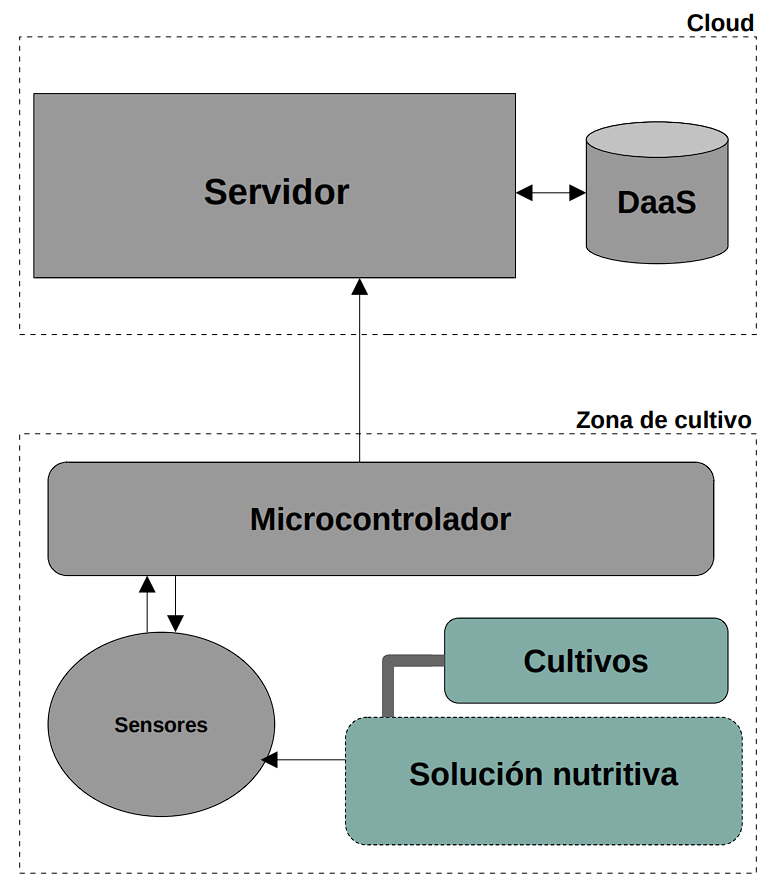
\includegraphics[width=.8\textwidth]{./Figures/Diagrama general de la solucion v2.png}
	\caption{Diagrama general de la solución.}
	\label{fig:diagramaGeneralDeLaSolucion}
\end{figure}